\documentclass[conference]{IEEEtran}
\IEEEoverridecommandlockouts
% The preceding line is only needed to identify funding in the first footnote. If that is unneeded, please comment it out.
%Template version as of 6/27/2024

\usepackage{ctex}
\usepackage{cite}
\usepackage{amsmath,amssymb,amsfonts}
\usepackage{algorithmic}
\usepackage{graphicx}
\usepackage{textcomp}
\usepackage{xcolor}
\def\BibTeX{{\rm B\kern-.05em{\sc i\kern-.025em b}\kern-.08em
    T\kern-.1667em\lower.7ex\hbox{E}\kern-.125emX}}
\begin{document}

\title{Conference Paper Title*\\
{\footnotesize \textsuperscript{*}Note: Sub-titles are not captured for https://ieeexplore.ieee.org  and
should not be used}
\thanks{Identify applicable funding agency here. If none, delete this.}
}

\author{\IEEEauthorblockN{1\textsuperscript{st} Given Name Surname}
\IEEEauthorblockA{\textit{dept. name of organization (of Aff.)} \\
\textit{name of organization (of Aff.)}\\
City, Country \\
email address or ORCID}
\and
\IEEEauthorblockN{2\textsuperscript{nd} Given Name Surname}
\IEEEauthorblockA{\textit{dept. name of organization (of Aff.)} \\
\textit{name of organization (of Aff.)}\\
City, Country \\
email address or ORCID}
\and
\IEEEauthorblockN{3\textsuperscript{rd} Given Name Surname}
\IEEEauthorblockA{\textit{dept. name of organization (of Aff.)} \\
\textit{name of organization (of Aff.)}\\
City, Country \\
email address or ORCID}
\and
\IEEEauthorblockN{4\textsuperscript{th} Given Name Surname}
\IEEEauthorblockA{\textit{dept. name of organization (of Aff.)} \\
\textit{name of organization (of Aff.)}\\
City, Country \\
email address or ORCID}
\and
\IEEEauthorblockN{5\textsuperscript{th} Given Name Surname}
\IEEEauthorblockA{\textit{dept. name of organization (of Aff.)} \\
\textit{name of organization (of Aff.)}\\
City, Country \\
email address or ORCID}
\and
\IEEEauthorblockN{6\textsuperscript{th} Given Name Surname}
\IEEEauthorblockA{\textit{dept. name of organization (of Aff.)} \\
\textit{name of organization (of Aff.)}\\
City, Country \\
email address or ORCID}
}

\maketitle

\begin{abstract}
This document is a model and instructions for \LaTeX.
This and the IEEEtran.cls file define the components of your paper [title, text, heads, etc.]. *CRITICAL: Do Not Use Symbols, Special Characters, Footnotes, 
or Math in Paper Title or Abstract.
\end{abstract}

\begin{IEEEkeywords}
component, formatting, style, styling, insert.
\end{IEEEkeywords}

\section{EXPERIMENTAL SETUP AND RESULTS (实验设置与结果分析)}

\subsection{Experimental Configuration (实验配置)}

\subsubsection{Topology and Infrastructure (拓扑与基础设施)}
实验采用三套异构边缘网络拓扑，节点资源配置对齐论文 A 与论文 B 的设置：

\begin{itemize}
    \item \textbf{小型拓扑 (Small)}: 15 个节点——5 个小型 (2GB, 10GFLOPS)、7 个中型 (4GB, 30GFLOPS)、3 个大型 (8GB, 100GFLOPS)
    \item \textbf{中型拓扑 (Medium)}: 30 个统一中型节点 (4GB, 30GFLOPS)
    \item \textbf{大型拓扑 (Large)}: 65 个节点（对齐论文 B 的 ta2 拓扑）
\end{itemize}

云边链路带宽为 100 Mbps，云边通信时延为 20 ms。每节点缓存容量 $K=10$ 个已部署架构。

\subsubsection{Traffic Models (流量模型)}
实验采用三种动态流量模式：

\begin{itemize}
    \item \textbf{Steady (稳态)}: 固定到达率 $\lambda=3.0$ req/s/节点
    \item \textbf{Tidal (潮汐)}: 周期性变化的到达率，模拟真实流量波动
    \item \textbf{Burst (突发)}: 高强度突发流量，测试系统在过载下的表现
\end{itemize}

基准 SLA 时延约束为 200 ms（jigsaw 任务为 100 ms）。

\subsubsection{Architecture Search Space (候选架构空间)}
候选架构来自预训练的超级网络，通过零成本代理（GSTC）评估生成 4096 个候选子网的属性三元组 $\langle S^{proxy}, P^{model}, F^{flops} \rangle$。7 种任务类型：class\_scene, class\_object, room\_layout, jigsaw, segmentsemantic, normal, autoencoder。

\subsection{Baseline Algorithms (基线算法)}

实验对比以下基线算法（均固定中等性能模型）：

\subsubsection{Paper A Baselines (TPDS 2023)}
\begin{itemize}
    \item \textbf{RLS} (Random Local Search): 随机局部搜索
    \item \textbf{FFD} (First Fit Decreasing): 首次适配降序
    \item \textbf{DRS} (Auto-scaling for Real-time Stream): 动态资源拆分
    \item \textbf{LEGO} (Joint optimization): 三阶段联合优化
\end{itemize}
路由策略：部署到平均距离最短的节点，采用 Dijkstra 最短路径路由。

\subsubsection{Paper B Baselines (TSC 2024)}
\begin{itemize}
    \item \textbf{GREEDY}: 贪心分配资源利用率最低节点 + 最近节点路由
    \item \textbf{PSO} (Particle Swarm Optimization): 粒子群优化
\end{itemize}

\subsubsection{Ablation Baselines (消融实验)}
\begin{itemize}
    \item \textbf{STATIC}: 固定 proxy\_score 最高架构
    \item \textbf{RESOURCE\_FIRST}: 仅 flops+params 最小优先
    \item \textbf{ACCURACY\_FIRST}: 仅 proxy\_score 最大优先
\end{itemize}

\subsection{Dynamic Model Replacement Mechanism (OURS 动态模型替换机制)}

OURS 算法实现了基于负载变化的动态模型替换机制：

\begin{enumerate}
    \item \textbf{初始化阶段}: 调用 \texttt{select\_arch()} 选择初始模型并缓存至 \texttt{deployed\_models}
    \item \textbf{运行时阶段}: 每次路由决策前，调用 \texttt{get\_deployed\_model()} 检测负载变化
    \item \textbf{替换判断}: 当负载变化超过 30\% 阈值时，触发 \texttt{\_should\_replace\_model()} 检查
    \item \textbf{模型替换}: 重新调用 \texttt{select\_arch()} 选择更适配当前负载的模型
\end{enumerate}

替换阈值定义：若 $last\_load > 0.1$，则 $load\_change = |current\_load - last\_load| / last\_load$；当 $load\_change > 0.3$ 时触发替换检查。

\subsection{Simulation Results (仿真结果)}

\subsubsection{Dynamic Load Experiments (动态负载实验)}
动态负载实验在 small/medium/large 三种拓扑下测试 steady、tidal、burst 三种流量模式。

评价指标：
\begin{itemize}
    \item \textbf{Avg E2E Latency (ms)}: 平均端到端时延
    \item \textbf{Success Rate}: 请求成功率
    \item \textbf{SLA Violation Rate}: SLA 违规率
    \item \textbf{Throughput (req/s)}: 系统吞吐量
    \item \textbf{Node Memory Utilization}: 节点内存利用率
\end{itemize}

\subsubsection{Perturbation Experiments (扰动实验)}
单变量扰动实验验证系统鲁棒性：

\begin{itemize}
    \item \textbf{到达率扰动}: $\lambda \in \{1, 2, 3, 5, 8, 12\}$ req/s
    \item \textbf{请求长度扰动}: $len \in \{2, 5, 10, 20, 50\}$ slots
    \item \textbf{请求类型数扰动}: $n_{task} \in \{1, 2, 3, 5, 7\}$
\end{itemize}

\subsubsection{Equal-Latency Resource Efficiency (等时延资源效率)}
在相同平均时延约束下，比较各算法的节点资源利用率差异。

\subsubsection{Scalability Analysis (规模扩展分析)}
在小（N=15）、中（N=30）、大（N=65）三种网络规模下评估算法性能随拓扑扩展的变化趋势。

\section{INTRODUCTION (引言)}

随着物联网（IoT）与 5G/6G 通信技术的快速发展，海量数据在网络边缘侧呈急剧增长趋势。为了满足自动驾驶、智能制造等时间敏感型应用的需求，边缘智能（Edge AI）应运而生，其致力于将深度学习模型以轻量化微服务（Microservices）的形式部署在靠近数据源的边缘节点上。然而，真实的边缘计算环境面临着显著的动态性挑战：一方面，异构边缘节点的物理资源（如算力、内存容量）受到严格限制；另一方面，网络中频繁涌现海量的、具有严格服务等级协议（SLA）的并发 AI 请求。这种高度动态的流量潮汐，要求边缘网络必须具备按需的模型编排与微服务动态调度能力。

为了给边缘节点提供适配其物理限制的高性能网络架构，神经架构搜索（NAS）技术被广泛应用。然而，现有基于 NAS 的边缘调度方案在面对真实的在线业务流时，暴露出严重的迟滞效应。传统 NAS 方法依赖计算密集的梯度训练迭代来获取模型的真实性能，搜索单个环境的最优架构往往耗费数百 GPU 小时。为了规避这一开销，现有的边缘框架普遍采用“离线预建池、在线静态匹配”的范式，即预先在云端耗费大量时间训练一个静态模型池，边缘节点仅负责查表匹配。然而，这种预设的静态模型池难以有效应对边缘环境高度突发的流量峰值：预设的高容量模型在流量突发时会导致计算资源过载及排队拥塞，而低容量模型在资源宽裕时又无法提供令人满意的推理精度。

为了缓解高昂搜索评估成本与边缘动态部署需求之间的矛盾，本文提出了一种基于云边协同的低延迟零成本 NAS 与动态启发式调度框架（Cloud-Edge Collaborative ZCP-NAS and Dynamic Heuristic Scheduling Framework）。本框架采用“云端超网预热，边缘低延迟搜索与拉取”的解耦范式。首先，云端离线预训练一个包含广阔搜索空间的超级网络（SuperNet）。当边缘节点面临流量波动时，系统在边缘侧低延迟触发“按需采样与快速评估”机制。我们依托无需训练的零成本代理（ZCP）模型，在毫秒级量化候选子网的精度潜力；同时，利用轻量级的物理特征解析器，快速完成对架构参数量（Params）与推理计算量（FLOPs）的特征提取。在此基础上，边缘调度器实时感知当前节点的瞬时可用内存与受流量严格制约的算力边界，执行低延迟的硬约束过滤，并利用动态启发式算法感知流量峰谷，自适应调整软约束权重。最终，边缘节点选出当前时隙的最优子网编码，按需从云端拉取对应的轻量级权重进行快速热重载部署。

本文的主要贡献总结如下：
\begin{itemize}
    \item 构建了一种面向云边协同的低延迟子网性能评估机制。本文引入并改进了基于图拓扑编码的零成本代理（GSTC），通过滤除耗时的张量反向传播，成功将密集的架构评估开销从系统的联合优化调度中有效解耦，实现了毫秒级的理论精度潜力输出，为模型下发与重载赢得了必要的传输时间窗口。
    \item 设计了硬约束驱动的动态启发式边缘调度算法。针对边缘节点异构且高度动态的状态，提出了一种多维过滤与动态加权机制。在硬约束层面，利用节点瞬时可用内存和受流量制约的算力红线进行安全过滤；在软约束层面，启发式算法通过感知实时并发流量变化，自适应调整选择权重，实现系统在面临流量洪峰时的“自适应降级（Adaptive Degradation）”，保障系统的整体吞吐量。
    \item 提出了轻量高可用的云边解耦部署流程。放宽了边缘节点需全量维持超网的存储假设，边缘侧仅运行极轻量的 ZCP 与结构解析器，决策后按需从云端拉取目标子网。该机制在保证较高服务可用性的同时，显著降低了异构边缘节点的存储与计算负担。
\end{itemize}

\section{SYSTEM ARCHITECTURE AND PROBLEM FORMULATION (系统架构与问题建模)}

本节提出一种面向严格时延 SLA 需求与异构物理约束的云边协同微服务按需编排框架。该框架将计算密集的模型训练卸载至云端，将轻量级的实时搜索与调度下放至边缘。

\subsection{System Modeling (系统建模)}

\subsubsection{云边协同与超网预训练 (Cloud-Edge Collaboration and SuperNet)}

假设边缘计算系统由云端中心服务器与一组地理分布式且物理资源异构的边缘节点集合 $\mathcal{N} = \{n_1, n_2, \dots, n_N\}$ 构成。为了避免在边缘节点进行高开销的模型训练，云端服务器在离线阶段预先训练了一个包含海量候选子网的超级网络（SuperNet）$\mathcal{W}$。该超网涵盖了不同深度、宽度和算子类型的丰富架构空间，供边缘节点按需查询与拉取。

在任意调度时隙 $t$，边缘节点 $n_i \in \mathcal{N}$ 的瞬时物理可用边界定义为二元组：
\begin{equation}
Node_i(t) = \langle M_i^{max}(t), C_i^{max} \rangle
\label{eq:node_state}
\end{equation}
其中，$M_i^{max}(t)$ 表示节点在时隙 $t$ 除去系统基础开销后，可用于部署 AI 模型的瞬时可用内存；$C_i^{max}$ 表示节点的峰值计算能力（以 FLOPS 衡量）。

\subsubsection{感知排队延迟的动态算力红线 (Queueing-Aware Dynamic Compute Constraint)}

在边缘网络中，AI 推理请求的到达率 $\lambda_i(t)$ 随时间呈潮汐波动。为了保障微服务的时间敏感性，系统设定了端到端的时延服务等级协议（SLA），记为 $T_{SLA}$。

请求的端到端延迟不仅包含模型前向推理时间，还受并发流量下的排队等待时间制约。对于任意候选子网架构 $a_k$，其在节点 $n_i$ 上的服务率近似为 $\mu_{i,k} = \frac{C_i^{max}}{F_k^{flops}}$。基于 M/M/1 排队系统理论，系统在时隙 $t$ 的平均响应时间应满足严格的 SLA 约束：
\begin{equation}
T_{req} = \frac{1}{\mu_{i,k} - \lambda_i(t)} = \frac{1}{\frac{C_i^{max}}{F_k^{flops}} - \lambda_i(t)} \le T_{SLA}
\label{eq:sla}
\end{equation}
经推导，为了保证在突发流量 $\lambda_i(t)$ 下系统维持稳定的排队状态，节点能够分配给目标子网的计算量上限（最大容忍计算量）$F_i^{max}(t)$ 需受到动态压缩：
\begin{equation}
F_i^{max}(t) = \frac{C_i^{max}}{\lambda_i(t) + \frac{1}{T_{SLA}}}
\label{eq:dynamic_compute_limit}
\end{equation}
公式 \eqref{eq:dynamic_compute_limit} 表明：当并发流量到达率上升时，边缘节点的算力红线将急剧收缩，从物理边界上迫使系统倾向于选择计算开销更小的轻量级模型，以抑制排队延迟的灾难性增长。

\subsubsection{在线架构属性元组 (On-the-fly Architecture Attributes)}

当时隙 $t$ 触发调度事件时，边缘调度引擎对云端超网 $\mathcal{W}$ 的结构空间进行启发式采样。对于采样到的候选子网 $a_k$，边缘侧通过极低延迟的结构解析器与自适应代理，将其多维属性提取为三元组：
\begin{equation}
a_k = \langle S_k^{proxy}, P_k^{model}, F_k^{flops} \rangle
\label{eq:arch_tuple}
\end{equation}
其中，$S_k^{proxy}$ 为由上下文感知的零成本代理评估器输出的预测得分（表征与当前场景高度适配的理论精度潜力）；$P_k^{model}$ 为该子网的参数量（表征内存占用预期）；$F_k^{flops}$ 为该子网的浮点运算次数（表征推理耗时预期）。

\subsection{Problem Formulation (联合优化问题定义)}

定义布尔型决策变量 $x_{i,k}(t) \in \{0, 1\}$，表示在时隙 $t$ 是否为节点 $n_i$ 选择并从云端拉取子网架构 $a_k$（候选池总量记为 $K$）。全局调度问题被建模为面向多维约束的在线联合优化问题：
\begin{align}
\max_{\mathbf{X}} \quad & \sum_{t=1}^{T} \sum_{i=1}^{N} \sum_{k=1}^{K} x_{i,k}(t) \cdot S_k^{proxy} \label{eq:opt_obj} \\
\text{s.t.} \quad & \sum_{k=1}^{K} x_{i,k}(t) = 1, \quad \forall i \in \mathcal{N}, \forall t \label{eq:opt_c1} \\
& \sum_{k=1}^{K} x_{i,k}(t) \cdot P_k^{model} \le M_i^{max}(t), \quad \forall i \in \mathcal{N}, \forall t \label{eq:opt_c2} \\
& \sum_{k=1}^{K} x_{i,k}(t) \cdot F_k^{flops} \le F_i^{max}(t), \quad \forall i \in \mathcal{N}, \forall t \label{eq:opt_c3}
\end{align}
约束 \eqref{eq:opt_c1} 保证单节点在当前时隙仅激活唯一的最优架构；约束 \eqref{eq:opt_c2} 与 \eqref{eq:opt_c3} 分别确保所选子网的资源需求不超出节点的瞬时可用内存与公式 \eqref{eq:dynamic_compute_limit} 限定的动态算力红线。
\section{ON-THE-FLY ZERO-COST ARCHITECTURE EVALUATION (边缘低延迟零成本评估)}

为了使得“边搜-云拉-边署”的云边协同流水线满足严格的实时性要求，系统必须在边缘侧极速完成对候选架构的多维属性评估，从而生成包含精度潜力与资源开销的属性三元组 $a_k = \langle S_k^{proxy}, P_k^{model}, F_k^{flops} \rangle$。由于候选子网 $a_k$ 的计算量（$F_k^{flops}$）与参数量（$P_k^{model}$）在其次级算子拓扑确定时即为恒定值，边缘调度器仅需通过 $\mathcal{O}(L)$ 复杂度的轻量级静态拓扑遍历，即可确定性地获取这两项物理开销特征。因此，本节将核心聚焦于如何规避昂贵的在线梯度训练，在极低延迟下实现精准且贴合边缘异构场景的模型精度潜力评估（$S_k^{proxy}$）。

传统零成本代理往往采用“一刀切”的静态指标，难以适应边缘计算环境中复杂多变的硬件约束与流量潮汐。为此，本框架引入了基于信息量量化编码的零成本代理（GSTC），并提出了面向边缘异构状态的自适应改装机制。

当边缘调度器生成候选子网 $a_k$ 的有向无环图（DAG）后，评估器利用本地缓存的算子信息保留率（$\eta$），极速提取出刻画网络拓扑信息流转的四个基础物理量：架构总路径信息量 $G$、路径信息差 $S$、输出节点接收总信息量 $T$ 以及输出节点接收信息差 $C$。为了使代理评估天然契合当前边缘节点的瞬时物理红线与业务需求，系统通过动态分配各组件的权重 $(\alpha, \beta, \gamma, \delta)$，甚至执行维度的裁剪，计算出自适应代理得分：
\begin{equation}
S_k^{proxy} = \alpha \cdot G + \beta \cdot S + \gamma \cdot \widehat{T} + \delta \cdot \widehat{C}
\label{eq:adaptive_gstc}
\end{equation}
其中，$\widehat{T}$ 与 $\widehat{C}$ 为基于全局搜索空间上下界的最大最小归一化项。得益于该评估机制的高度可扩展性，调度器能够根据节点实时感知的多维状态，动态映射至与之最契合的定制化方案，以下例举了三种最具代表性的典型场景：

\textbf{算力极简与极低延迟场景 (Low-Latency \& Resource-Constrained Scheme)：} 
当边缘节点面临极端的物理资源受限或正处于高并发流量洪峰时，复杂的网络拓扑虽然能提升信息差，但会引发严重的内存碎片化与不可预测的访存延迟。此时，系统触发降维裁剪机制，将结构差异项的权重强行置零（即 $\beta = \delta = 0$），甚至对总信息量 $G$ 引入负向衰减惩罚。该方案剥离了对网络复杂度的鼓励机制，从评估源头引导调度器倾向于选择层数较浅、拓扑较简的候选架构，从而最大化系统的吞吐量与抗过载能力。

\textbf{算力宽裕与高精度需求场景 (High-Accuracy \& Relaxed-Latency Scheme)：} 
针对算力相对宽裕且对推理精度要求极高的节点，系统的首要优化目标转换为模型的表征能力。物理量 $G$ 与 $\widehat{T}$ 与网络的深度和特征提取
容量高度正相关。因此，系统赋予总信息量与输出信息量极高的权重因子（即 $\alpha, \gamma \gg 1$）。该方案能够捕获搜索空间内信息流转无损耗、层级结构极深的高复杂度子网，确保在资源允许的边界内榨干硬件的每一分算力以换取极致的精度。

\textbf{常态化稳健均衡场景 (Balanced Robust Scheme)：} 
在节点资源与流量处于平稳状态时，系统采用全量评估组件与均衡权重（$\alpha=\beta=\gamma=\delta=1$）。该方案兼顾了网络的深度（由 $G, T$ 表征）与残差结构的多样性（由 $S, C$ 表征），在理论精度潜力与结构冗余度之间取得最优的综合折中，提供高鲁棒性的常态化候选集。

通过上述自适应机制，系统将繁重的在线联合优化问题巧妙地前置解耦。边缘节点在毫秒级内即可生成不仅符合物理红线，且其拓扑特性天然贴合瞬时业务场景的多维候选架构集，为后续从云端按需拉取模型争取了极大的时间裕度。

\section{CLOUD-EDGE COLLABORATIVE HEURISTIC DEPLOYMENT (云边协同按需调度与自适应降级)}

在边缘侧获取了上下文感知的架构属性三元组后，边缘调度器随即执行基于瞬时环境的单次（Single-shot）动态调度决策。如果说前文的零成本代理改装实现了“拓扑级”的场景适配，那么本节的启发式调度则旨在应对边缘环境高度突发的微观状态波动，实现“定量级”的资源自适应降级与部署。具体而言，该调度机制被无缝整合为一个包含硬约束过滤、启发式加权选择以及按需拉取的三阶段流水线。

首先，在多维物理红线过滤阶段，调度引擎面对当前时隙生成的候选子网集合 $\mathcal{A}$，基于瞬时物理红线执行 $\mathcal{O}(|\mathcal{A}|)$ 复杂度的严格安全过滤。一方面，系统执行内存红线过滤，剔除满足 $P_k^{model} > M_i^{max}(t)$ 的子网，绝对杜绝由内存溢出（OOM）导致的边缘节点系统故障；另一方面，系统执行排队时延红线过滤，剔除满足 $F_k^{flops} > F_i^{max}(t)$ 的高计算需求子网。该约束结合了前文推导的排队论模型，确保当前选择的推理计算量在突发到达率 $\lambda_i(t)$ 下，依然能满足严格的 SLA 时延边界。过滤完成后，系统成功将全局搜索空间安全裁剪为满足当前时隙硬约束的实时候选子集 $\mathcal{A}_i^*(t)$。

随后，调度流程进入动态启发式自适应降级阶段。为了在候选子集 $\mathcal{A}_i^*(t)$ 的多维冲突特征（理论精度潜力、真实推理延迟与内存占用）中取得最优折中，本文设计了基于全局边界归一化（Global Boundary Normalization）的效用函数：
\begin{equation}
U(a_k) = w_1(t) \cdot \widehat{S}_k^{proxy} - w_2(t) \cdot \widehat{F}_k^{flops} - w_3(t) \cdot \widehat{P}_k^{model}
\label{eq:utility_function}
\end{equation}
其中 $\widehat{(\cdot)}$ 表示基于云端超网全集上下界的最大最小归一化，以避免局部样本特征导致的尺度失真。此处引入的 $\widehat{S}_k^{proxy}$ 来源于前文基于节点属性定向改装的 GSTC 变体输出，已天然具备拓扑亲和性。为了应对极其频繁的微观流量潮汐，权重向量由瞬时并发流量 $\lambda_i(t)$ 与资源水位实时映射驱动：
\begin{equation}
\begin{aligned}
    w_2(t) &= \alpha \cdot \exp\left( \max\left(0, \frac{\lambda_i(t) - \lambda_{th}}{\lambda_{th}}\right) \right), \\
    w_3(t) &= \beta \cdot \frac{M_{used}(t)}{M_{total}}
\end{aligned}
\label{eq:dynamic_weights}
\end{equation}
且满足归一化精度权重 $w_1(t) = \frac{1}{1 + w_2(t) + w_3(t)}$，其中 $\lambda_{th}$ 为节点预标定的临界安全流量阈值。该动态加权机制通过严密的逻辑应对不同的边缘环境状态。在稳态寻优（Steady-State Optimization）场景下，当实时流量 $\lambda_i(t) \le \lambda_{th}$ 时，时延惩罚 $w_2(t)$ 维持在基础常量水平，调度器充分信任 GSTC 代理评估的精度潜力，倾向于拉取理论得分更高、表征能力更强的架构。相反，在抗过载自适应降级（Overload-Resistant Adaptive Degradation）场景下，当瞬时并发流量突破阈值即 $\lambda_i(t) > \lambda_{th}$ 时，公式 \eqref{eq:dynamic_weights} 触发指数级增长，导致时延与计算量惩罚 $w_2(t)$ 显著放大并压制精度权重 $w_1(t)$。此时，算法主动触发系统级“软降级”，牺牲部分模型精度以换取参数量与计算量极小的轻量级架构，从而确保节点在面临流量洪峰时依然维持高吞吐量与服务可用性。

最后，在云边协同按需拉取与重载阶段，调度器计算出当前时隙的最优子网 $a^* = \arg\max_{a_k \in \mathcal{A}_i^*(t)} U(a_k)$ 后，向云端发送该子网的唯一结构编码（Architecture Encoding）。云端服务器随即从预训练的超网 $\mathcal{W}$ 中快速切分出对应的轻量级权重，并下发至边缘。得益于自适应 GSTC 在评估阶段节省的巨大搜索开销，整个“搜索-决策-拉取”流水线耗时被严格压缩，系统能够在有效的容忍时间窗口内完成边缘节点的热重载部署（Hot-Reload Deployment），真正实现真实动态环境下的微服务按需敏捷编排。



\section{Introduction}
This document is a model and instructions for \LaTeX.
Please observe the conference page limits. For more information about how to become an IEEE Conference author or how to write your paper, please visit   IEEE Conference Author Center website: https://conferences.ieeeauthorcenter.ieee.org/.

\subsection{Maintaining the Integrity of the Specifications}

The IEEEtran class file is used to format your paper and style the text. All margins, 
column widths, line spaces, and text fonts are prescribed; please do not 
alter them. You may note peculiarities. For example, the head margin
measures proportionately more than is customary. This measurement 
and others are deliberate, using specifications that anticipate your paper 
as one part of the entire proceedings, and not as an independent document. 
Please do not revise any of the current designations.

\section{Prepare Your Paper Before Styling}
Before you begin to format your paper, first write and save the content as a 
separate text file. Complete all content and organizational editing before 
formatting. Please note sections \ref{AA} to \ref{FAT} below for more information on 
proofreading, spelling and grammar.

Keep your text and graphic files separate until after the text has been 
formatted and styled. Do not number text heads---{\LaTeX} will do that 
for you.

\subsection{Abbreviations and Acronyms}\label{AA}
Define abbreviations and acronyms the first time they are used in the text, 
even after they have been defined in the abstract. Abbreviations such as 
IEEE, SI, MKS, CGS, ac, dc, and rms do not have to be defined. Do not use 
abbreviations in the title or heads unless they are unavoidable.

\subsection{Units}
\begin{itemize}
\item Use either SI (MKS) or CGS as primary units. (SI units are encouraged.) English units may be used as secondary units (in parentheses). An exception would be the use of English units as identifiers in trade, such as ``3.5-inch disk drive''.
\item Avoid combining SI and CGS units, such as current in amperes and magnetic field in oersteds. This often leads to confusion because equations do not balance dimensionally. If you must use mixed units, clearly state the units for each quantity that you use in an equation.
\item Do not mix complete spellings and abbreviations of units: ``Wb/m\textsuperscript{2}'' or ``webers per square meter'', not ``webers/m\textsuperscript{2}''. Spell out units when they appear in text: ``. . . a few henries'', not ``. . . a few H''.
\item Use a zero before decimal points: ``0.25'', not ``.25''. Use ``cm\textsuperscript{3}'', not ``cc''.)
\end{itemize}

\subsection{Equations}
Number equations consecutively. To make your 
equations more compact, you may use the solidus (~/~), the exp function, or 
appropriate exponents. Italicize Roman symbols for quantities and variables, 
but not Greek symbols. Use a long dash rather than a hyphen for a minus 
sign. Punctuate equations with commas or periods when they are part of a 
sentence, as in:
\begin{equation}
a+b=\gamma\label{eq}
\end{equation}

Be sure that the 
symbols in your equation have been defined before or immediately following 
the equation. Use ``\eqref{eq}'', not ``Eq.~\eqref{eq}'' or ``equation \eqref{eq}'', except at 
the beginning of a sentence: ``Equation \eqref{eq} is . . .''

\subsection{\LaTeX-Specific Advice}

Please use ``soft'' (e.g., \verb|\eqref{Eq}|) cross references instead
of ``hard'' references (e.g., \verb|(1)|). That will make it possible
to combine sections, add equations, or change the order of figures or
citations without having to go through the file line by line.

Please don't use the \verb|{eqnarray}| equation environment. Use
\verb|{align}| or \verb|{IEEEeqnarray}| instead. The \verb|{eqnarray}|
environment leaves unsightly spaces around relation symbols.

Please note that the \verb|{subequations}| environment in {\LaTeX}
will increment the main equation counter even when there are no
equation numbers displayed. If you forget that, you might write an
article in which the equation numbers skip from (17) to (20), causing
the copy editors to wonder if you've discovered a new method of
counting.

{\BibTeX} does not work by magic. It doesn't get the bibliographic
data from thin air but from .bib files. If you use {\BibTeX} to produce a
bibliography you must send the .bib files. 

{\LaTeX} can't read your mind. If you assign the same label to a
subsubsection and a table, you might find that Table I has been cross
referenced as Table IV-B3. 

{\LaTeX} does not have precognitive abilities. If you put a
\verb|\label| command before the command that updates the counter it's
supposed to be using, the label will pick up the last counter to be
cross referenced instead. In particular, a \verb|\label| command
should not go before the caption of a figure or a table.

Do not use \verb|\nonumber| inside the \verb|{array}| environment. It
will not stop equation numbers inside \verb|{array}| (there won't be
any anyway) and it might stop a wanted equation number in the
surrounding equation.

\subsection{Some Common Mistakes}\label{SCM}
\begin{itemize}
\item The word ``data'' is plural, not singular.
\item The subscript for the permeability of vacuum $\mu_{0}$, and other common scientific constants, is zero with subscript formatting, not a lowercase letter ``o''.
\item In American English, commas, semicolons, periods, question and exclamation marks are located within quotation marks only when a complete thought or name is cited, such as a title or full quotation. When quotation marks are used, instead of a bold or italic typeface, to highlight a word or phrase, punctuation should appear outside of the quotation marks. A parenthetical phrase or statement at the end of a sentence is punctuated outside of the closing parenthesis (like this). (A parenthetical sentence is punctuated within the parentheses.)
\item A graph within a graph is an ``inset'', not an ``insert''. The word alternatively is preferred to the word ``alternately'' (unless you really mean something that alternates).
\item Do not use the word ``essentially'' to mean ``approximately'' or ``effectively''.
\item In your paper title, if the words ``that uses'' can accurately replace the word ``using'', capitalize the ``u''; if not, keep using lower-cased.
\item Be aware of the different meanings of the homophones ``affect'' and ``effect'', ``complement'' and ``compliment'', ``discreet'' and ``discrete'', ``principal'' and ``principle''.
\item Do not confuse ``imply'' and ``infer''.
\item The prefix ``non'' is not a word; it should be joined to the word it modifies, usually without a hyphen.
\item There is no period after the ``et'' in the Latin abbreviation ``et al.''.
\item The abbreviation ``i.e.'' means ``that is'', and the abbreviation ``e.g.'' means ``for example''.
\end{itemize}
An excellent style manual for science writers is \cite{b7}.

\subsection{Authors and Affiliations}\label{AAA}
\textbf{The class file is designed for, but not limited to, six authors.} A 
minimum of one author is required for all conference articles. Author names 
should be listed starting from left to right and then moving down to the 
next line. This is the author sequence that will be used in future citations 
and by indexing services. Names should not be listed in columns nor group by 
affiliation. Please keep your affiliations as succinct as possible (for 
example, do not differentiate among departments of the same organization).

\subsection{Identify the Headings}\label{ITH}
Headings, or heads, are organizational devices that guide the reader through 
your paper. There are two types: component heads and text heads.

Component heads identify the different components of your paper and are not 
topically subordinate to each other. Examples include Acknowledgments and 
References and, for these, the correct style to use is ``Heading 5''. Use 
``figure caption'' for your Figure captions, and ``table head'' for your 
table title. Run-in heads, such as ``Abstract'', will require you to apply a 
style (in this case, italic) in addition to the style provided by the drop 
down menu to differentiate the head from the text.

Text heads organize the topics on a relational, hierarchical basis. For 
example, the paper title is the primary text head because all subsequent 
material relates and elaborates on this one topic. If there are two or more 
sub-topics, the next level head (uppercase Roman numerals) should be used 
and, conversely, if there are not at least two sub-topics, then no subheads 
should be introduced.

\subsection{Figures and Tables}\label{FAT}
\paragraph{Positioning Figures and Tables} Place figures and tables at the top and 
bottom of columns. Avoid placing them in the middle of columns. Large 
figures and tables may span across both columns. Figure captions should be 
below the figures; table heads should appear above the tables. Insert 
figures and tables after they are cited in the text. Use the abbreviation 
``Fig.~\ref{fig}'', even at the beginning of a sentence.

\begin{table}[htbp]
\caption{Table Type Styles}
\begin{center}
\begin{tabular}{|c|c|c|c|}
\hline
\textbf{Table}&\multicolumn{3}{|c|}{\textbf{Table Column Head}} \\
\cline{2-4} 
\textbf{Head} & \textbf{\textit{Table column subhead}}& \textbf{\textit{Subhead}}& \textbf{\textit{Subhead}} \\
\hline
copy& More table copy$^{\mathrm{a}}$& &  \\
\hline
\multicolumn{4}{l}{$^{\mathrm{a}}$Sample of a Table footnote.}
\end{tabular}
\label{tab1}
\end{center}
\end{table}

\begin{figure}[htbp]
\centerline{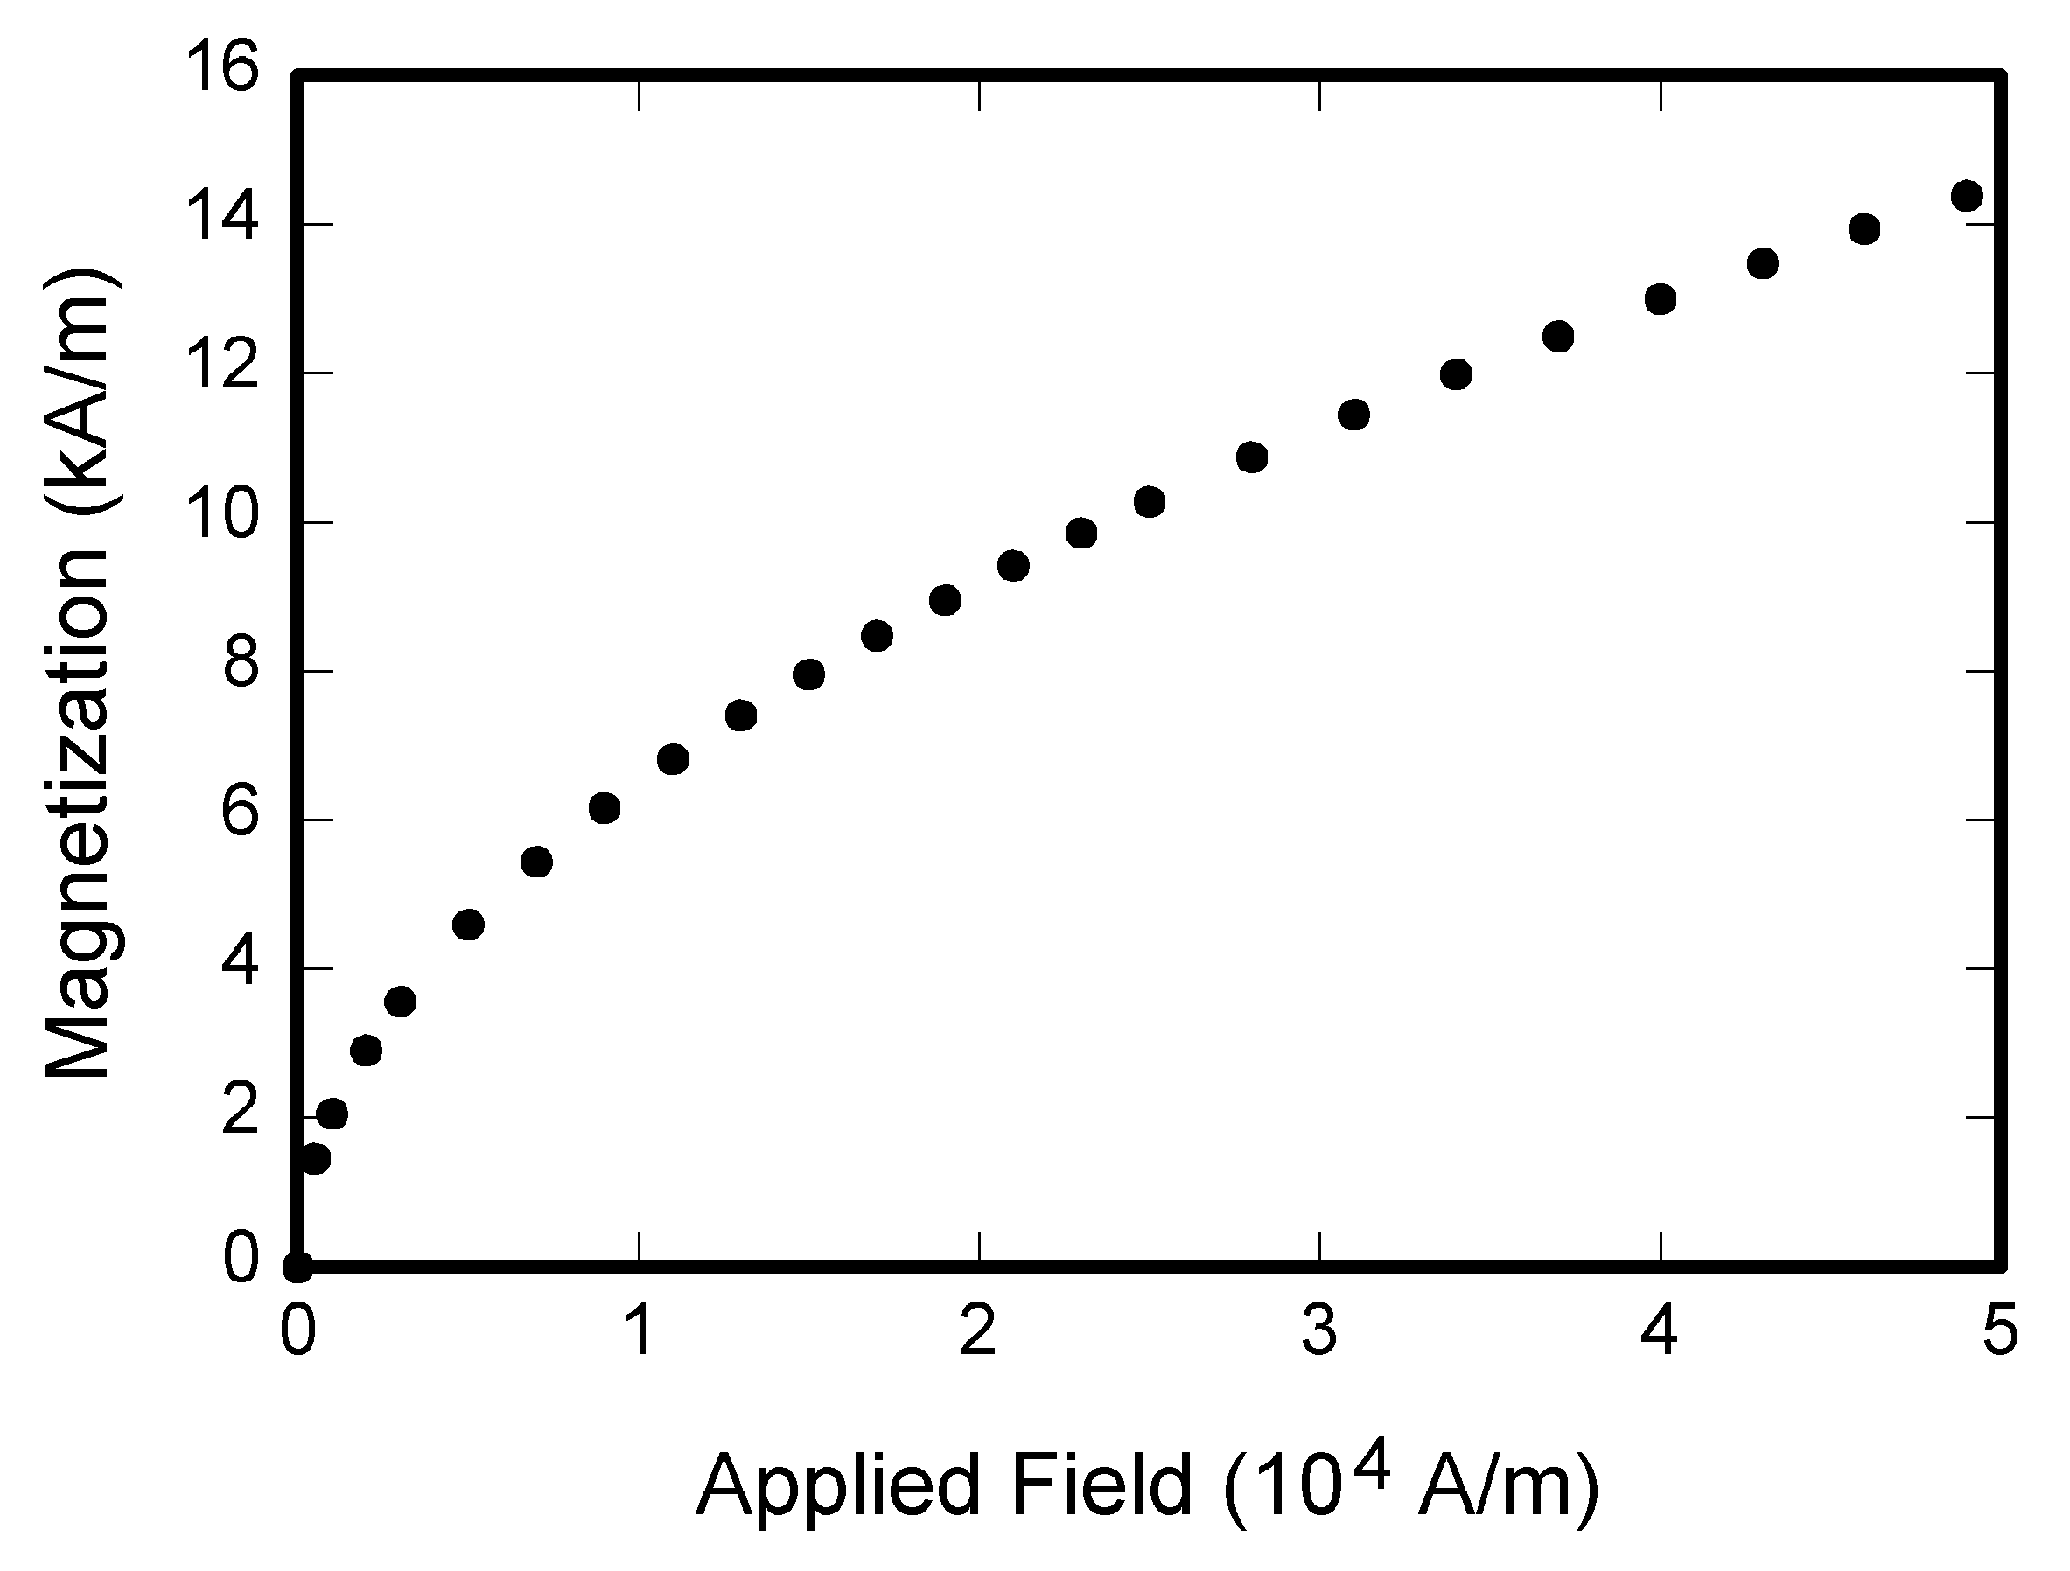
\includegraphics{fig1.png}}
\caption{Example of a figure caption.}
\label{fig}
\end{figure}

Figure Labels: Use 8 point Times New Roman for Figure labels. Use words 
rather than symbols or abbreviations when writing Figure axis labels to 
avoid confusing the reader. As an example, write the quantity 
``Magnetization'', or ``Magnetization, M'', not just ``M''. If including 
units in the label, present them within parentheses. Do not label axes only 
with units. In the example, write ``Magnetization (A/m)'' or ``Magnetization 
\{A[m(1)]\}'', not just ``A/m''. Do not label axes with a ratio of 
quantities and units. For example, write ``Temperature (K)'', not 
``Temperature/K''.

\section*{Acknowledgment}

The preferred spelling of the word ``acknowledgment'' in America is without 
an ``e'' after the ``g''. Avoid the stilted expression ``one of us (R. B. 
G.) thanks $\ldots$''. Instead, try ``R. B. G. thanks$\ldots$''. Put sponsor 
acknowledgments in the unnumbered footnote on the first page.

\section*{References}

Please number citations consecutively within brackets \cite{b1}. The 
sentence punctuation follows the bracket \cite{b2}. Refer simply to the reference 
number, as in \cite{b3}---do not use ``Ref. \cite{b3}'' or ``reference \cite{b3}'' except at 
the beginning of a sentence: ``Reference \cite{b3} was the first $\ldots$''

Number footnotes separately in superscripts. Place the actual footnote at 
the bottom of the column in which it was cited. Do not put footnotes in the 
abstract or reference list. Use letters for table footnotes.

Unless there are six authors or more give all authors' names; do not use 
``et al.''. Papers that have not been published, even if they have been 
submitted for publication, should be cited as ``unpublished'' \cite{b4}. Papers 
that have been accepted for publication should be cited as ``in press'' \cite{b5}. 
Capitalize only the first word in a paper title, except for proper nouns and 
element symbols.

For papers published in translation journals, please give the English 
citation first, followed by the original foreign-language citation \cite{b6}.

\begin{thebibliography}{00}
\bibitem{b1} G. Eason, B. Noble, and I. N. Sneddon, ``On certain integrals of Lipschitz-Hankel type involving products of Bessel functions,'' Phil. Trans. Roy. Soc. London, vol. A247, pp. 529--551, April 1955.
\bibitem{b2} J. Clerk Maxwell, A Treatise on Electricity and Magnetism, 3rd ed., vol. 2. Oxford: Clarendon, 1892, pp.68--73.
\bibitem{b3} I. S. Jacobs and C. P. Bean, ``Fine particles, thin films and exchange anisotropy,'' in Magnetism, vol. III, G. T. Rado and H. Suhl, Eds. New York: Academic, 1963, pp. 271--350.
\bibitem{b4} K. Elissa, ``Title of paper if known,'' unpublished.
\bibitem{b5} R. Nicole, ``Title of paper with only first word capitalized,'' J. Name Stand. Abbrev., in press.
\bibitem{b6} Y. Yorozu, M. Hirano, K. Oka, and Y. Tagawa, ``Electron spectroscopy studies on magneto-optical media and plastic substrate interface,'' IEEE Transl. J. Magn. Japan, vol. 2, pp. 740--741, August 1987 [Digests 9th Annual Conf. Magnetics Japan, p. 301, 1982].
\bibitem{b7} M. Young, The Technical Writer's Handbook. Mill Valley, CA: University Science, 1989.
\bibitem{b8} D. P. Kingma and M. Welling, ``Auto-encoding variational Bayes,'' 2013, arXiv:1312.6114. [Online]. Available: https://arxiv.org/abs/1312.6114
\bibitem{b9} S. Liu, ``Wi-Fi Energy Detection Testbed (12MTC),'' 2023, gitHub repository. [Online]. Available: https://github.com/liustone99/Wi-Fi-Energy-Detection-Testbed-12MTC
\bibitem{b10} ``Treatment episode data set: discharges (TEDS-D): concatenated, 2006 to 2009.'' U.S. Department of Health and Human Services, Substance Abuse and Mental Health Services Administration, Office of Applied Studies, August, 2013, DOI:10.3886/ICPSR30122.v2
\bibitem{b11} K. Eves and J. Valasek, ``Adaptive control for singularly perturbed systems examples,'' Code Ocean, Aug. 2023. [Online]. Available: https://codeocean.com/capsule/4989235/tree
\end{thebibliography}

\vspace{12pt}
\color{red}
IEEE conference templates contain guidance text for composing and formatting conference papers. Please ensure that all template text is removed from your conference paper prior to submission to the conference. Failure to remove the template text from your paper may result in your paper not being published.

\end{document}
